LOcal Rule-based Explainer (LORE), introduced by Guidotti et al.\cite{guidotti2019lore}, addresses several fundamental limitations of LIME and SHAP by shifting from feature importance to \textit{symbolic decision rules}. The original LORE employs a genetic algorithm for neighborhood generation, creating a more faithful and dense representation of the local decision space compared to LIME's random sampling approach \cite{bodria2023benchmarking}. $\text{LORE}_{sa}$ extends this foundation with enhanced stability and actionability features.

% \textbf{Core Mechanism:}
LORE and $\text{LORE}_{sa}$'s core mechanism is that given a black-box model $b$ and instance $x$ with prediction $b(x) = y$ the methods generate synthetic neighborhoods through genetic optimization. However, while the original LORE generates a single neighborhood $Z$ and trains one decision tree classifier $g$, $\text{LORE}_{sa}$ generates multiple neighborhoods and employs a bagging-like approach, creating N decision trees that are subsequently merged into a single interpretable predictor. From the resulting decision tree structure, both methods extract (i) a \textit{factual decision rule} corresponding to the path followed by instance $x$ to reach decision $y$, and (ii) a set of \textit{counterfactual rules} indicating conditions that would alter the prediction outcome. $\text{LORE}_{sa}$ enhances the counterfactual extraction with actionability constraints, filtering rules based on user-specified constraints $U$ on immutable features \cite{guidotti2022stable, bodria2023benchmarking}.

\begin{algorithm}[H]
\label{alg:LORE_sa}
\caption{$\text{LORE}_{sa}$(x, b, K, U)}
\KwIn{$x$ - instance to explain, $b$ - black-box, $K$ - knowledge, $U$ - constr.}
\KwOut{$e$ - (counter)factual explanation of $x$}
$D \leftarrow \emptyset$ \tcp*{init. empty set of decision trees}
\For{$i \in \{1, \ldots, N\}$}{
    $Z^{(i)}_{=} \leftarrow$ genetic$(x, \text{fitness}_{x=}, b, K)$ \tcp*{neighborhood generation}
    $Z^{(i)}_{\neq} \leftarrow$ genetic$(x, \text{fitness}_{x\neq}, b, K)$ \tcp*{neighborhood generation}
    $Z^{(i)} \leftarrow Z_{=} \cup Z_{\neq}$ \tcp*{merge neighborhoods}
    $Y^{(i)} \leftarrow b(Z^{(i)})$ \tcp*{apply black-box}
    $d^{(i)} \leftarrow$ buildDecisionTree$(Z^{(i)}, Y^{(i)})$ \tcp*{build decision tree}
    $D \leftarrow D \cup \{d^{(i)}\}$ \tcp*{add decision tree to list}
}
$c \leftarrow$ mergeDecisionTrees$(D)$ \tcp*{merge decision trees}
$r = (p \rightarrow y) \leftarrow$ extractDecisionRule$(c, x)$ \tcp*{factual rule}
$\Phi \leftarrow$ extractCounterfactuals$(c, r, x, U)$ \tcp*{extract actionable counterfactual}
\Return{$e \leftarrow r, \Phi$}\;
\end{algorithm}

% \textbf{Genetic Neighborhood Generation:} 
Unlike LIME's random perturbation, $\text{LORE}_{sa}$ use genetic algorithms that optimize neighborhood generation through fitness functions (\ref{eq:fitnessLORE_sa1} and \ref{eq:fitnessLORE_sa2}) that minimize distances to the decision boundary \cite{guidotti2022stable}. This approach yields neighborhoods that are denser in boundary regions, providing more accurate approximations of local black-box behavior compared to uniform random generation. Figure \ref{fig:LORE_sa_black_box_boundary} demonstrates that genetic approaches produce neighborhoods with better decision boundary characterization \cite{guidotti2022stable}.

\begin{equation} 
\label{eq:fitnessLORE_sa1}
\text{fitness}^x_=(z)=I_{x\neq}+d(x,z)+l(b_p(x),b_p(z))
\end{equation}

\begin{equation} 
\label{eq:fitnessLORE_sa2}
\text{fitness}^x_=(z)=I_{x\neq}+d(x,z)+(1-l(b_p(x),b_p(z)))
\end{equation}

\subsection{Neighborhood Generation}

The quality of neighborhood generation is a critical factor in determining the fidelity and reliability of local explanations. The synthetic neighborhood around the explained instance has to accurately capture the local decision boundary of the black-box model while maintaining sufficient density and diversity to allow surrogate model training. $\text{LORE}_{sa}$'s approach to neighborhood generation represents a significant improvement from traditional random sampling methods, using a genetic algorithm to optimize the quality and representativeness of the generated synthetic instances.

\subsubsection{Genetic Algorithm for Neighborhood Generation}

$\text{LORE}_{sa}$ employs a genetic algorithm, shown in Alghorithm \ref{alg:geneticAlgoLORE_sa} specifically designed to overcome the limitations of random sampling by optimizing neighborhood quality through evolutionary computation principles \cite{guidotti2022stable}. The genetic approach treats neighborhood generation as an optimization problem where the fitness of generated instances is evaluated based on their contribution to accurate local decision boundary approximation.

\begin{algorithm}[ht]
\caption{genetic(x, fitness, b, K)}
\label{alg:geneticAlgoLORE_sa}
\SetKwInOut{KwParams}{Parameters}
\KwIn{$x$ - instance to explain, fitness - fitness function, $b$ - black-box, $K$ - knowledge base}
\KwParams{$n$ - population size, $g$ - nbr of generations, $p_c$ - prob crossover, $p_m$ - prob mutation}
\KwOut{$Z$ - neighbors of $x$}
$P_0 \leftarrow (x | \forall 1, \ldots, n)$; $i \leftarrow 0$ \tcp*{population init.}
\While{$i < g$}{
    $P' \leftarrow$ crossover$(P_i, p_c)$ \tcp*{mix records}
    $P'' \leftarrow$ mutate$(P', p_m, K)$ \tcp*{perform mutations}
    $S \leftarrow$ evaluate$(P'', \text{fitness}, b)$ \tcp*{evaluate population}
    $P_{i+1} \leftarrow$ select$(P'', S)$ \tcp*{select sub-population}
    $i \leftarrow i + 1$ \tcp*{update population}
}
$Z \leftarrow P_i$\;
\Return{$Z$}\;
\end{algorithm}

Figure \ref{fig:LORE_sa_black_box_boundary} illustrates the differences between uniform random generation and genetic optimization for a black-box consisting of a random forest model on a bi-dimensional feature space \cite{guidotti2022stable}. The genetic approach yields a neighborhood that is denser in the boundary region of the predictor, while random generation produces scattered instances that fail to adequately characterize the decision boundary \cite{guidotti2022stable}.

% \textbf{Fitness Function Design:} 
The genetic algorithm employs two complementary fitness functions to generate balanced neighborhoods. For instances with the same class as the target ($Z_=^i$), the fitness function $\text{fitness}^{x}_{=}(z)$ (\ref{eq:fitnessLORE_sa1}) optimizes the proximity to the target instance while maintaining the same classification outcome. Conversely, for instances with different classes ($Z_{\neq}^i$), the fitness function $\text{fitness}^{x}_{\neq}(z)$ (\ref{eq:fitnessLORE_sa2}) seeks instances that are close to the target but receive different predictions from the black-box model \cite{guidotti2022stable}. This dual-objective approach ensures that the neighborhood contains both confirmatory instances (supporting the original decision) and contrastive instances (illustrating alternative outcomes).

% \textbf{Evolutionary Optimization Process:} 
The genetic algorithm iteratively evolves populations of candidate instances through standard genetic operations, including selection, crossover, and mutation. The selection process favors instances with higher fitness scores, promoting the survival of instances that better serve the explanation objectives. Crossover operations combine successful instances to explore new regions of the feature space, while mutation introduces controlled randomness to prevent premature convergence and maintain diversity \cite{guidotti2022stable}.

% \textbf{Knowledge-Informed Mutation:} 
A key innovation in $\text{LORE}_{sa}$'s genetic approach involves the integration of domain knowledge through the knowledge base $K$, which contains information about feature distributions, including "domain of admissible values, mean, variance, probability distribution, etc.". This knowledge base guides the mutation process to ensure that generated instances remain consistent with realistic feature distributions, preventing the creation of implausible or out-of-distribution synthetic instances that would compromise explanation quality \cite{guidotti2022stable}.

\subsubsection{Comparative Analysis of Neighborhood Generation Methods}

As previously introduced Figure \ref{fig:LORE_sa_black_box_boundary} illustrates the differences between uniform random generation and genetic optimization for a black-box consisting of a random forest model on a bi-dimensional feature space \cite{guidotti2022stable}. The genetic approach "yields a neighborhood that is denser in the boundary region of the predictor", while random generation produces scattered instances that fail to adequately characterize the decision boundary \cite{guidotti2022stable}.

\begin{figure}
    \centering
    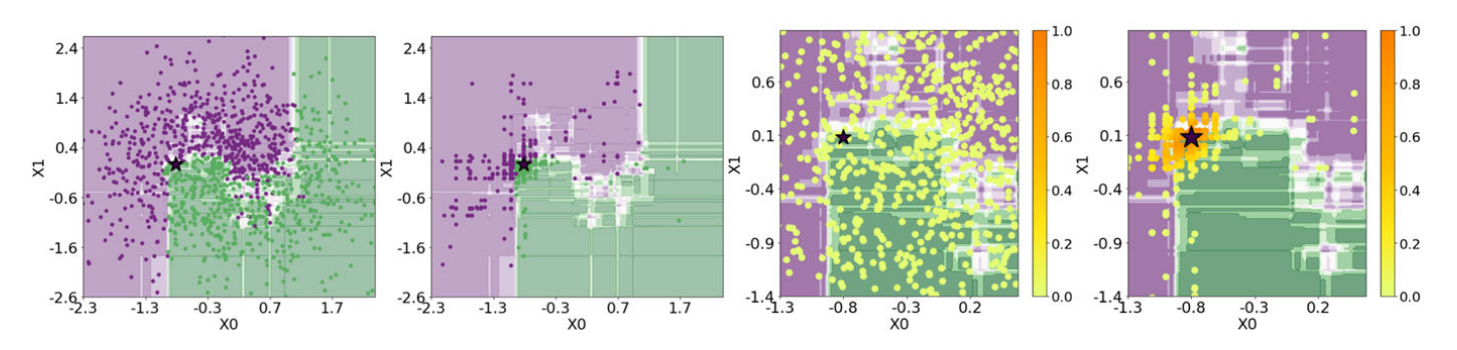
\includegraphics[width=0.9\linewidth]{images/LORE_sa_black_box_boundary.png}
    \caption{Black-box boundary: purple versus green. Starred instance x. UniforMachine Learningy random (1st) and genetic (2nd) neighborhoods. In the (3rd) and (4th) plot is reported the density with levels in the bar}
    \label{fig:LORE_sa_black_box_boundary}
\end{figure}

% \textbf{Density and Boundary Characterization:} 
The genetic approach produces neighborhoods with superior density characteristics in critical decision regions. "The density of the generated instances is a key factor in extracting correct and faithful local interpretable predictors and explanations" \cite{guidotti2022stable}. By concentrating instances near the decision boundary, the genetic algorithm enables more accurate approximation of the black-box model's local behavior, resulting in higher-fidelity surrogate models.

% \textbf{Variability Reduction:} 
Unlike random sampling, "the genetic approach of $\text{LORE}_{sa}$ is driven by minimization of the fitness functions, hence less variable neighborhoods are generated" \cite{guidotti2022stable}. This reduced variability contributes directly to improved explanation consistency, addressing one of the fundamental challenges in local explanation methods. The optimization-driven approach ensures that repeated explanation generation for the same instance produces consistent results, improving user trust and system reliability.

\subsubsection{Multi-Neighborhood Ensemble Strategy}

$\text{LORE}_{sa}$ extends the genetic neighborhood generation approach through a sophisticated ensemble strategy that addresses the consistency challenges inherent in local explanation methods. Rather than relying on a single neighborhood, $\text{LORE}_{sa}$ generates multiple independent neighborhoods $Z = \{Z^{(1)}, Z^{(2)}, \ldots, Z^{(N)}\}$ through repeated genetic optimization \cite{guidotti2022stable}.
% 
% \textbf{Bagging-Inspired Approach:} 
The multi-neighborhood strategy draws inspiration from ensemble learning techniques, particularly bagging methods that achieve improved predictive performance and consistency through aggregation. 
Each neighborhood $Z^{(i)}$ is generated independently using the genetic algorithm, providing diverse perspectives on the local decision space.

% \textbf{Decision Tree Ensemble Construction:} 
For each generated neighborhood $Z^{(i)}$, $\text{LORE}_{sa}$ constructs a decision tree classifier $d^{(i)}$ trained on instances labeled with black-box predictions. The algorithm then merges these multiple decision trees into a single interpretable predictor $c$ through a tree merging process \cite{guidotti2022stable}. This ensemble approach leverages the consistency benefits of averaging multiple predictors while maintaining the interpretability advantages of tree-based models.

% \textbf{Consistency Enhancement:} 
The multi-neighborhood ensemble strategy directly addresses the inconsistency issues that plague single-neighborhood approaches. "Bagging, boosting, and random forests achieve high predictive performances, which, in our context, means high fidelity (accuracy w.r.t. black-box decisions). Moreover, they achieve consistency of predictions by averaging the decisions of several trees" \cite{guidotti2022stable}. By adopting those principles, $\text{LORE}_{sa}$ achieves both improved fidelity and enhanced consistency in explanation generation.

\subsubsection{Technical Implementation and Parameter Optimization}
The practical implementation of genetic neighborhood generation involves careful consideration of multiple algorithmic parameters that influence both computational efficiency and explanation quality. $\text{LORE}_{sa}$ employs the DEAP (Distributed Evolutionary Algorithms in Python) \cite{Fortin2012DEAPEA} framework for genetic algorithm implementation, utilizing optimized CART \cite{ClassificationandRegressionTrees, IntroductiontoDataMining} decision tree construction through scikit-learn for efficiency \cite{guidotti2022stable}.

% \textbf{Key Parameters:} 
The genetic algorithm operates with several critical parameters: neighborhood size, crossover probability, mutation probability, and number of generations \cite{guidotti2022stable}. These parameters have been empirically confirmed to provide optimal trade-offs between explanation quality and computational efficiency across diverse datasets and model types.

% \textbf{Scalability Considerations:} 
While genetic neighborhood generation requires greater computational resources compared to random sampling, the approach remains practically viable for real-world applications. 
The investment in computational resources yields substantial returns in explanation quality, fidelity, and consistency.

The genetic neighborhood generation approach in $\text{LORE}_{sa}$ represents a fundamental advancement in local explanation methodology, addressing critical limitations of random sampling while providing theoretically motivated and empirically confirmed improvements in explanation quality. The integration of evolutionary optimization principles with domain knowledge and ensemble strategies represents a robust foundation for generating high-quality synthetic neighborhoods that enable accurate and stable local explanations.

\subsection{Rule Extraction}

The transformation of complex decision tree structures into human-interpretable symbolic rules represents the last step in $\text{LORE}_{sa}$'s explanation generation process. Once the genetic algorithm has produced high-quality synthetic neighborhoods and multiple decision trees have been merged into a single interpretable predictor, $\text{LORE}_{sa}$ employs rule extraction techniques to derive both factual and counterfactual explanations that capture the logic underlying the involved black-box model decisions.

\subsubsection{Conceptual Foundation of Symbolic Rule Extraction}

The choice of decision trees as the interpretable surrogate model in $\text{LORE}_{sa}$ is fundamentally motivated by their natural capacity for symbolic reasoning \cite{guidotti2022stable}. Unlike feature importance methods that provide numerical weights, decision trees enable direct extraction of logical rules through their hierarchical structure. "The choice of decision trees as interpretable predictors allows for symbolic reasoning: (i) factual decision rules can readily be derived from the root-to-leaf path in a tree; and, (ii) counterfactual rules can be extracted by symbolic reasoning over a decision tree" \cite{guidotti2022stable, Breiman1984ClassificationAR, 10.1609/aaai.v33i01.330110035}.

% Source: Factual and Counterfactual Explanations for BlackBox Decision Making lore 2019.pdf, Referenced as Figure 4
\begin{figure}[ht]
\centering
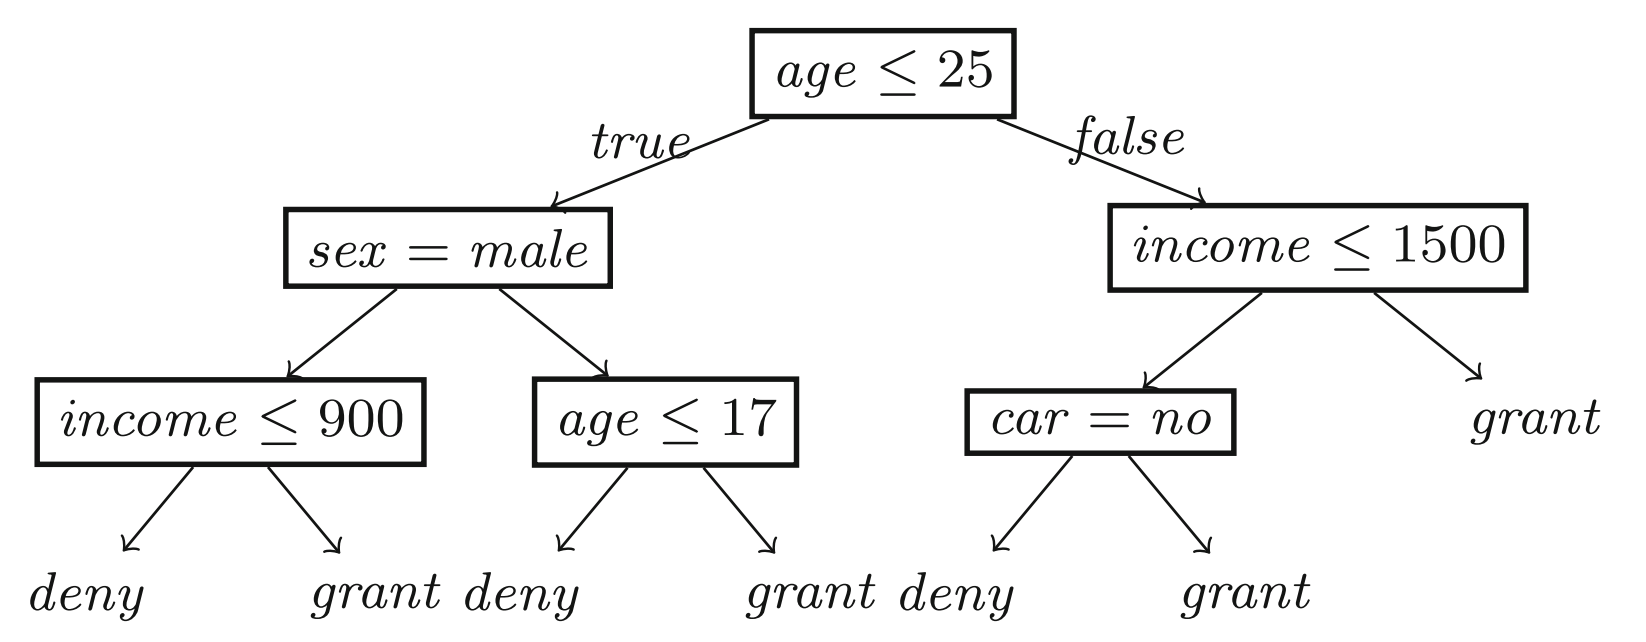
\includegraphics[width=0.6\textwidth]{images/decision tree example lore_sa.png}
\caption{Decision tree mimicking the local behavior of a black box classifier. The tree shows split conditions leading to grant/deny loan decisions, illustrating how factual and counterfactual rules can be extracted from root-to-leaf paths.}
\label{fig:decision_tree_example}
\end{figure}

Decision rules provide explanations that are fundamentally closer to human reasoning patterns compared to feature importance approaches \cite{bodria2023benchmarking}. A decision rule $r$ takes the form $p \rightarrow y$, where $p$ represents a premise composed of Boolean conditions on feature values, and $y$ denotes the consequence or predicted class \cite{guidotti2022stable}. The premise $p$ consists of a conjunction of split conditions of the form $a_i \in [v_i^{(l)}, v_i^{(u)}]$, where $a_i$ represents a feature and $v_i^{(l)}, v_i^{(u)}$ denote lower and upper bound values in the domain of $a_i$ extended with $\pm\infty$ \cite{guidotti2022stable}.

An instance $x$ satisfies rule $r$, or $r$ covers $x$, if every Boolean condition in premise $p$ evaluates to true for $x$ \cite{guidotti2022stable}. When the instance to be explained satisfies $p$, the rule $p \rightarrow y$ represents a candidate explanation of the decision $c(x)$, and if the interpretable predictor accurately mimics the black-box behavior in the neighborhood of $x$, the rule constitutes a valid local explanation of $b(x) = c(x) = y$ \cite{bodria2023benchmarking}.

\subsubsection{Factual Rule Extraction Process}

The extraction of factual rules from the merged decision tree $c$ follows a systematic path-tracing procedure that captures the logical sequence of decisions leading to the predicted outcome. Given the decision tree $c$ and the instance $x$ to be explained, the factual rule $r = p \rightarrow y$ is constructed by "including in $p$ the split conditions on the path from the root to the leaf satisfied by $x$, and setting $y = c(x) = b(x)$" \cite{guidotti2022stable}.

This path-based extraction ensures that the factual rule is both consistent with the decision tree structure and satisfied by the target instance $x$. The set of split conditions encountered along the root-to-leaf path, also referred to as a \textit{direct reason}, provides a complete logical characterization of why the instance received its particular classification \cite{guidotti2022stable}. Unlike minimal explanation approaches that seek to reduce rule complexity, $\text{LORE}_{sa}$ prioritizes comprehensiveness, as "experiments show $\text{LORE}_{sa}$ returns very small rules" naturally without requiring further minimization procedures \cite{guidotti2022stable}.

% \textbf{Example of Factual Rule:} 
An example of a factual rul is illustrated in Figure \ref{fig:decision_tree_example}; consider an instance $x=\{\text{age}=22, \text{sex}=\text{male}, \text{income}=800, \text{car}=\text{no}\}$ from a credit risk assessment system where $\text{LORE}_{sa}$ generates the factual rule: $\{\text{age} \leq 25, \text{sex} = \text{male}, \text{income} \leq 900\} \rightarrow \text{deny}$. This rule explicitly states that the loan denial is attributed to the conjunction of being 25 years old or younger, being male, and having an income of 900 or less. The factual explanation provides transparent insight into exactly which feature combinations drove the black-box decision \cite{guidotti2022stable}.

\subsubsection{Counterfactual Rule Extraction Algorithm}

Counterfactual rule extraction represents a more sophisticated procedure that identifies alternative decision paths within the decision tree that would result in different classification outcomes. $\text{LORE}_{sa}$ employs Algorithm \ref{alg:extractCounterfactuals} to systematically discover and rank counterfactual rules based on minimality criteria \cite{guidotti2022stable}.

\begin{algorithm}[ht]
\caption{extractCounterfactuals(c, r, x, U)}
\label{alg:extractCounterfactuals}
\KwIn{$c$ - decision tree, $r$ - rule, $x$ - instance to explain, $U$ - constraints}
\KwOut{$\Phi$ - set of counterfactual rules for $p$}
$Q \leftarrow$ getPathsWithDifferentLabel$(c, y)$ \tcp*{get paths with $y \neq \hat{y}$}
$\Phi \leftarrow \emptyset$; $\min \leftarrow +\infty$ \tcp*{initialize counterfactual set}
\For{$q \in Q$}{
    \If{\textbf{not} $q \rightarrow U|q$}{
        \textbf{continue} \tcp*{skip rule if constraints not satisfied}
    }
    $q_{len} \leftarrow nf(q, x) = |\{sc \in q \mid \neg sc(x)\}|$\;
    
    \If{$q_{len} < \min$}{
        $\Phi \leftarrow \{q \rightarrow y\}$; $\min \leftarrow q_{len}$\;
    }
    \ElseIf{$q_{len} = \min$}{
        $\Phi \leftarrow \Phi \cup \{q \rightarrow y\}$\;
    }
}
\Return{$\Phi$}\;
\end{algorithm}

The counterfactual extraction process operates through the following systematic approach:

\textbf{Path Identification:} The algorithm first identifies all paths in the decision tree $c$ that lead to decisions $y' \neq y$, where $y$ represents the original prediction for instance $x$. For each such path, the conjunction of split conditions $q$ forms a potential counterfactual premise \cite{guidotti2022stable}.

\textbf{Minimality Ranking:} Critical to the usefulness of counterfactual explanations is the principle of minimality. The algorithm ranks potential counterfactual rules $q \rightarrow y'$ by computing $\text{qlen} = \text{nf}(q, x) = |\{sc \in q \mid \neg sc(x)\}|$, which counts the number of split conditions in $q$ that are not satisfied by the original instance $x$ \cite{guidotti2022stable}. This metric directly corresponds to the number of feature changes required to achieve the alternative outcome.

\textbf{Constraint Satisfaction:} To ensure actionability, the algorithm filters counterfactual candidates based on user-specified constraints $U$ on features. "Since both the premise $q$ and the constraints $U$ are logic formulae, the test amounts at checking validity of the implication $q \rightarrow U|_q$" \cite{guidotti2022stable}. This constraint satisfaction step eliminates counterfactuals that involve changing immutable features (such as age decreasing or demographic characteristics) or violate domain-specific restrictions.

Continuing the credit risk example shown in Figure \ref{fig:decision_tree_example}, $\text{LORE}_{sa}$ might generate counterfactual rules such as $\{\text{age}>25, \text{income} > 1500\} \rightarrow \text{grant}$ and $\{\text{income} \leq1500, \text{car} = \text{yes}\} \rightarrow \text{grant}$ \cite{guidotti2022stable}. These counterfactuals explicitly indicate that either having an income greater than 1500 and being older than 25 or having an income lower than 1500 and owning a car would result in loan approval, providing actionable insights into how the prediction could be altered.

\subsubsection{Decision Tree Ensemble Merging for Rule Extraction}

A crucial innovation in $\text{LORE}_{sa}$ involves the extraction of rules from merged decision tree ensembles rather than individual trees. The multi-neighborhood approach generates multiple decision trees $\{d^{(1)}, d^{(2)}, \ldots, d^{(N)}\}$ that are merged into a single interpretable predictor $c$ before rule extraction can proceed \cite{guidotti2022stable}.

% \textbf{Tree Merging Methodology:} 
$\text{LORE}_{sa}$ adopts the merging approach introduced by Fan et al.\cite{Fan2020ClassificationAV}, which implements a two-phase procedure for combining multiple decision trees into a unified structure \cite{guidotti2022stable}. The first phase merges decision regions using a recursive approach based on condition trees, while the second phase performs pruning to reduce complexity by removing inner nodes with identical leaf classifications.
% 
% \textbf{Lossless Information Preservation:} 
A critical advantage of this merging approach is its lossless nature, "the merging method maintains for every instance the class label assigned by the tree ensembles" \cite{guidotti2022stable}. This preservation ensures that rule extraction from the merged tree precisely reflects the collective decision logic of the ensemble.

% \textbf{Consistency Enhancement:} 
The ensemble merging process directly contributes to explanation consistency by reducing the effects of randomness in neighborhood generation. "The generalized representation of the knowledge contained in the multiple decision trees helps in reducing the probability that small changes in the data may result in very different explanations" \cite{guidotti2022stable}. This consistency improvement represents a significant advantage over single-tree approaches that may be sensitive to variations in neighborhood composition.

% Source: Stable and actionable explanations of blackbox models through factual and counterfactual rules.pdf, Multiple pages
\begin{table}[ht]
    \centering
    \caption{Aggregated evaluation metrics over experimental datasets and black-boxes showing performance comparison between different explanation methods. $\text{LORE}_{sa}$ achieves the best performance in most metrics including fidelity, complexity, and stability measures. Bold value indicates the best perfomance}
    \label{tab:lore_sa_performance}
    \begin{adjustbox}{width=\textwidth,center}
    \begin{tabular}{lrrrrr}
        \hline
        Method & Silhouette & Fidelity & Complexity & Instability & $\text{Instability}_{si}$ \\
        \hline
        anchor & .116 ± .51 & .912 ± .21 & 4.950 ± 8.20 & .174 ± 0.29 & .651 ± .949 \\
        brl & .019 ± .30 & .869 ± .09 & 1.998 ± 1.23 & .889 ± 0.45 & n.a. \\
        lime & .444 ± .49 & .904 ± .23 & 9.733 ± 1.47 & .787 ± 1.58 & .159 ± .142 \\
        lore & .408 ± .49 & .996 ± .01 & 4.917 ± 3.69 & .123 ± 0.22 & .259 ± .847 \\
        maple & .127 ± .56 & .949 ± .09 & 29.014 ± 3.25 & .651 ± 1.66 & n.a. \\
        shap & .463 ± .56 & n.a. & 6.070 ± 3.84 & .608 ± 0.58 & \textbf{.017 ± .052} \\
        $\text{LORE}_{sa}$ & \textbf{.569 ± .46} & .992 ± .20 & 3.986 ± 3.93 & \textbf{.073 ± 0.07} & .107 ± .081 \\
        $\text{LORE}^d_{sa}$ & \textbf{.569 ± .46} & \textbf{.999 ± .01} & 5.105 ± 4.29 & .083 ± 0.08 & .107 ± .066 \\
        \hline
        \hline
        Metric & anchor & LORE & brl & \textbf{$\text{LORE}_{sa}$} & \textbf{$\text{LORE}_{sa}^d$} \\
        \hline
        coverage & .284 ± .32 & .492 ± .27 & .344 ± .30 & \textbf{.742 ± .27} & .485 ± .26 \\
        \hline
        precision & .912 ± .21 & .993 ± .07 & .732 ± .22 & .772 ± .26 & \textbf{.998 ± .02} \\
        \hline
        h-mean & .433 ± .25 & .657 ± .11 & .468 ± .25 & \textbf{.694 ± .25} & .615 ± .22 \\
        \hline
    \end{tabular}
    \end{adjustbox}
\end{table}

\subsubsection{Advantages of Rule-Based Explanations}
The symbolic rule extraction approach employed by $\text{LORE}_{sa}$ offers several compelling advantages over alternative explanation formats, as demonstrated by the performance metrics in Table \ref{tab:lore_sa_performance}:

\textbf{Human Cognitive Alignment:} "Rule-based explanations are considered closer to human reasoning w.r.t. the feature importance-based explanations" \cite{bodria2023benchmarking}. Logical rules align naturally with human decision-making processes, making them more intuitive for non-expert users to understand and confirm.

\textbf{Logical Transparency:} Unlike feature importance vectors that require domain expertise to interpret, symbolic rules provide explicit logical conditions that clearly specify decision boundaries. Users can directly verify whether rule conditions apply to their specific circumstances and understand the logical chain leading to predictions.

\textbf{Actionable Insights:} Counterfactual rules provide direct guidance on how to achieve different outcomes by specifying exact feature changes required. This actionability is particularly valuable in applications where users seek to understand how to modify their situation to achieve favorable predictions.

\textbf{Completeness and Precision:} Rule-based explanations capture complete logical conditions for decisions rather than partial information conveyed through feature importance rankings. This completeness ensures that users receive a comprehensive understanding of the decision logic rather than incomplete glimpses into the model behavior.

\textbf{Superior Performance Metrics:} As shown in Table \ref{tab:lore_sa_performance}, $\text{LORE}_{sa}$ achieves the best overall performance across multiple evaluation dimensions, with particularly strong results in fidelity (0.992), low complexity (3.986), and great stability (0.073 instability score), significantly outperforming traditional methods like LIME and SHAP.

\subsection{Current LORE Approach for Showing the Extracted Rules and Counterfactual Rules}\label{subsec:currentLOREapproach}

The current implementation of $\text{LORE}_{sa}$ presents explanations through a structured data format that arranges all relevant information for understanding both factual and counterfactual reasoning in seven primary components that together provide a comprehensive view of the local decision space around the explained instance.

\subsubsection{Factual Rule Representation}

The factual rule component represents the logical path that leads to the predicted outcome for the target instance. The rule structure follows a premise-consequence format where:

\begin{itemize}
    \item \textbf{Premises}: A list of conditions, each specifying an attribute (\texttt{attr}), a threshold value (\texttt{val}), and a comparison operator (\texttt{op})
    \item \textbf{Consequence}: The predicted class outcome with its corresponding attribute and equality operator
\end{itemize}

For example, a factual rule might be represented as:
\begin{verbatim}
'rule': {
    'premises': [{'attr': 'capital-gain', 'val': 7148.0, 'op': '>'}],
    'consequence': {'attr': 'income', 'val': '>50K', 'op': '='}
}
\end{verbatim}

This structure explicitly states that instances with capital gain greater than 7148.0 are predicted to have income greater than 50K, providing the user with direct logical understanding of the decision boundary.

\subsubsection{Counterfactual Rule Representation}

Counterfactual rules follow an identical structural format but represent alternative decision paths that would yield different classification outcomes. Each counterfactual rule specifies the minimal set of feature changes required to alter the prediction, formatted as:

\begin{verbatim}
'counterfactuals': [{
    'premises': [
        {'attr': 'capital-gain', 'val': 7148.0, 'op': '<='},
        {'attr': 'capital-loss', 'val': 2728.5, 'op': '<='},
        {'attr': 'age', 'val': 57.0, 'op': '<='},
        {'attr': 'hours-per-week', 'val': 59.0, 'op': '<='}
    ],
    'consequence': {'attr': 'income', 'val': '<=50K', 'op': '='}
}]
\end{verbatim}

The counterfactual representation directly indicates that individuals with capital gain at or below 7148.0, capital loss at or below 2728.5, age at or below 57, and working 59 hours per week or fewer would be predicted to earn 50K or less.

\subsubsection{Supporting Information Components}

Beyond the core rule structures, $\text{LORE}_{sa}$ provides additional components to allow users to better understand the generated explanations:

\textbf{Fidelity Score}: A numerical measure (ranging from 0 to 1) indicating how accurately the surrogate decision tree approximates the black-box model's behavior in the local neighborhood. High fidelity scores (approaching 1.0) indicate reliable explanations.

\textbf{Delta Specifications}: The \texttt{deltas} component explicitly identifies the minimal changes required for counterfactual outcomes, formatted as logical conditions such as \texttt{[[\{'att': 'capital-gain', 'op': '<=', 'thr': 7148.0\}]]}.

\textbf{Counterfactual Samples and Predictions}: The \texttt{counterfactual\_samples} and \texttt{counterfactual\_predictions} components work in tandem to provide both the synthetic instances generated through the genetic algorithm and their corresponding black-box model predictions. The \texttt{counterfactual\_samples} array contains concrete examples of alternative scenarios that maintain the same feature structure as the original dataset while representing variations that lead to different predictions. Each synthetic instance in this array has a corresponding entry in the \texttt{counterfactual\_predictions} array, which lists the black-box model's actual predictions for that instance. This paired structure enables verification of counterfactual logic and assessment of neighborhood quality by allowing direct comparison between the generated instances and their predicted outcomes.

\textbf{Feature Importance Ranking}: A ranked list of features with their corresponding importance scores, providing complementary insight into which attributes most significantly influence local decision boundaries.

\subsubsection{Limitations of Current Presentation Format}

While the structured data format provides comprehensive information, it presents several limitations for practical explainability that deserve closer examination. Most immediately, there is the considerable \textbf{cognitive load} placed on users attempting to parse and understand the textual representation. This challenge is particularly acute for those without technical backgrounds, who must mentally compose logical conditions to completely grasp decision scenarios, task that demands substantial mental effort and can be overwhelming.
Beyond this, users might face the struggle of developing a contextual understanding of what they're seeing without the ability to easily \textbf{visualize} how the explained instance relates to the \textbf{decision boundaries}. Users are left somewhat in the dark about the density and distribution of the generated synthetic neighborhood that supports the explanation. This lack of perspective makes it difficult to assess whether the explanation represents a typical case or an outlier, and whether the supporting evidence is robust or sparse.
The static nature of the current information delivery further complicates the situation. With no mechanism for interactive exploration, users cannot investigate how variations in \textbf{specific features might affect both factual and counterfactual rules}. This becomes especially problematic when we consider scalability challenges. As datasets grow more complex, involving higher dimensions or intricate decision boundaries with multiple interacting features, the textual representation becomes increasingly difficult to comprehend.
